\chapter{ZigBee}

ZigBee is widely used in various fields from home automation to Mars exploration; it is considered the ``cousin'' of Bluetooth: they are standardized by the same company and can coexist.

\begin{paracol}{2}

   \colfill
   Aside from the application layer, ZigBee defines also a \textit{Network Layer} which perfectly matches and maps to the underlying MAC and Physical Layers, standardized by \texttt{IEEE 802.15.4};
   ZigBee is built on top of such IEEE standard.
   \colfill

   \switchcolumn
   
   \begin{figure}[htbp]
      \centering
      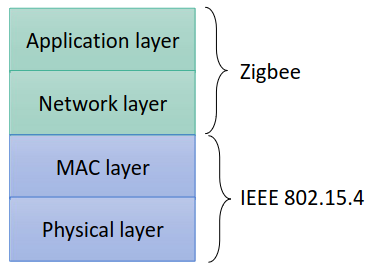
\includegraphics{images/zigbee_layers.png}
      \caption{ZigBee layers}
      \label{fig:zigbee_layers}
   \end{figure}
\end{paracol}

\labelitemize{\textit{Key Features}}{
   \begin{itemize}
      \item Specification of the physical and MAC layers for low-rate Wireless Personal Area Networks (PAN)
      \item Infrastructure-less
      \item Short range
      \item Support for star and peer-to-peer topologies
      \item Can coexist with IEEE 802.11 and IEEE 802.15.1 (Bluetooth)
      \item Works on licence-free frequency bands
   \end{itemize}
}